\documentclass[main.tex]{subfiles}
\begin{document}
    \section{Implementation of Android User Interface}
        In order to develop an acceptable user interface for the Android version of the application, a variety of packages and custom made
        components were implemented. This section aims to explain the implementation of the user interface in detail, discussing each component
        individually.
        \subsection{Defining Interface Layout}
	        In Android applications, the layout of the user interface is defined by writing code into an AXML file. This code is similar to
            XML, but here tags are used to place elements into the layout and specify the values of various options e.g. colour.
            In our case, each tab in the interface displays its own layout.
            These layouts are linear (elements are placed one after the other), and contain various built-in Android components, as well
            as several components of our own design, all of which will be discussed in this section. Thankfully, Xamarin Studio contains a 
            User Interface Designer which grants the ability to create interfaces by dragging and dropping desired components from a menu
            of options. Once this process is complete, the designer then generates the equivalent AXML code, making the development process
            much easier as one can see the end result without having to compile and deploy the whole application. In some edge cases it was necessary
            to hand modify certain parts of the AXML, but this was a fairly trivial task.
        \subsection{Managing Separate Interface Pages}
            The main method of separating disjoint pages of the user interface was achieved through the use of a tab based system. This was chosen due
            to both intuitive usability and ease of implementation. In order to make the addition of new tabs easier to code, an extension class,
            \texttt{ActionBarExtensions}, was developed which contained a function that automates the process of adding a new tab to the
            interface. This function takes the tab name as its first argument. Its other argument is an anonymous function that handles any behaviour
            that must be executed upon accessing the tab. For example, selecting the `debug' tab changes the value of the variable \texttt{inDebug} to
            true. Note that the final release version of the application will contain less tabs due to the lack of need for the end user to be able to access
            such a page. The setup of all of the tabs is handled by a call to \texttt{setUpUITabs}, which creates tabs for the main screen, settings, and 
            debugging information relating to the step counter in order to facilitate testing.
        \subsection{Destination Selection Menu}
            In order to improve the user experience, a drop down menu (in Android development terms this is known as a \texttt{Spinner}) that contains
            all possible destinations was added to the interface. Items in the menu consist of a destination name and some of the following items,
            where applicable:
            \begin{itemize}
                \item Occupier of the room.
                \item Type of the room e.g. office.
                \item Floor number.
            \end{itemize}
            The spinner is set up by passing it an object of type \texttt{Adapter}. Specifically, in our case, we pass in an \texttt{ArrayAdapter}, a sub-class of \texttt{Adapter}.
            This contains the elements
            that are used to populate the list. For us, this is a list of \texttt{Room} objects that were read in as input from an XML file as detailed in
            \textbf{[reference relevant section of report]}.
            This adapter is then set to a specific type of layout (currently this is set to simple). Once this has been done, the adapter is then bound to the spinner in order to display
            the correct values to the user. Finally, a callback function, \texttt{spinnerItemSelected}, was added to the spinner to specify the results of a user selecting a given item.
            This allows the user to select a destination from the menu, as when an item is selected, the correct destination coordinates are set within the application. This menu is shown within Figure ~\ref{fig:androidSpinner}.
       
            \begin{center}
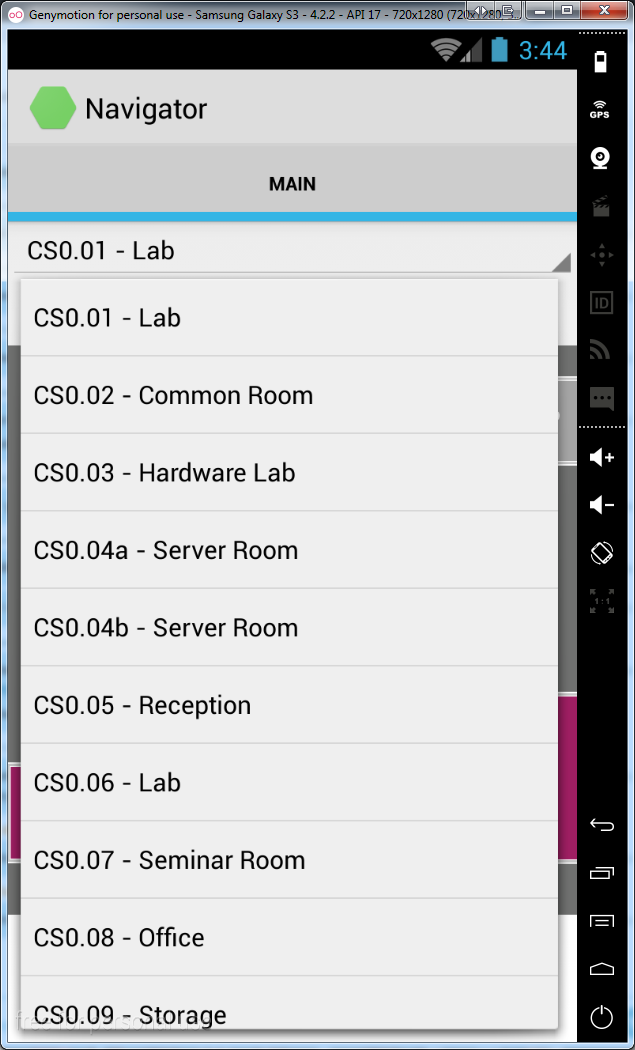
\includegraphics[scale=0.5]{images/search_open.png}
\captionof{figure}{Android room selection menu}
\label{fig:androidSpinner}
\end{center}
        \subsection{Displaying the Floor Plan}
            The vast majority of screen real estate on the main tab of the application is occupied by the image of the floor plan being displayed. Therefore, it was crucial to 
            implement this part of the interface in such a way that it is as simple and intuitive as possible, as the user will spend most of their time using this part of
            the application. By implementing standard features that make use of the touch screen functionality of smart phones (dragging the image around, pinch-to-zoom,
            pressing and holding etc.)
            the learning curve of the interface is greatly reduced as features such as these are extremely common in mobile applications. Therefore, this takes advantage of 
            what can be assumed to be pre-existing knowledge for most end users, reducing the need for excessive tutorials or instructions.
            
            One of the first key issues to handle was the problem that, due to the large size of the floor plan images being displayed (especially when zoomed in), it would need
            to be possible for the for the user to `scroll' through the image. Initially the Android frame \texttt{ScrollView} was used to contain the image. However, it was quickly
            discovered that this only allowed for scrolling in a single direction specified in the AXML code - horizontally or vertically.
            This was clearly insufficient for our purposes, so other methods
            were considered. The first potential fix was that of nesting another \texttt{ScrollView} inside the first, set to scroll in the direction that its parent did not.
            This did allow for scrolling in multiple directions to function, but only one at a time i.e. diagonal scrolling was not possible. In order to solve this problem,
            the Android development team examined various packages, but failed to find one that exactly suited our requirements. Therefore, a custom class
            (\texttt{CustomImageView}) was written to implement all of the desired functionality. This class is described in the section below.
            \subsubsection{CustomImageView Implementation}
                This part of the application is made up of two key classes, one simple, the other more complex. The first of these is the \texttt{CustomImageViewGestureDetector},
                which extends the basic \texttt{SimpleGestureListener} to work with our custom image view and handles the detection of common smartphone gestures. For our purposes,
                we implemented custom detection for touching the screen (known as a `down' gesture), double tapping on the screen, and pressing and holding down on the screen
                (from now on referred to as a `long press').
                
                The main bulk of the new functionality is contained within the \texttt{CustomImageView} class itself. As with all programs that handle image translation and scaling,
                the class contains a matrix that can be applied to carry out translations and zooms on the displayed image (rotations were not required). The class contains functionality
                that allows this matrix to be accessed and applied. Section \ref{subsec:MapMaker} shows this matrix in action when points are translated into correct positions.
                There is also functionality to set the image to be displayed as either a specific bitmap or an Android resource.
                
                The custom behaviours were implemented by monitoring for touch events on the device
                screen. When a touch is detected its coordinates are stored as the position of the `last move'.
                If the `touch count' is at least two (more than one finger is being used, therefore the user is performing either
                a pinch or its inverse), the action was judged to be a scale and the relevant flag was set in the class. If this flag is set, the distance between the two points of contact
                is used to calculate the value by which to scale the image being displayed. This scale is then posted to the image matrix, which is then applied to the image in
                order to carry out the zoom action. Note that if the action would scale the image outside of the bounds specified by the minimum or maximum allowed zoom,
                the scale would stop at these boundary values. Therefore continuing to `pinch' at this point has no effect on the interface. The double tap motion could also be
                used to zoom to the maximum or minimum amount instantly, however this was handled slightly differently. In this case there is no need to calculate a scale
                factor based on movements as the minimum/maximum values are already known. Therefore, the zoom was executed using this known value and the
                (\textit{x, y}) coordinates of the double tap action.
                If the motion was not deemed to be a scale (only one finger is used by the user to perform the motion), the start and end points
                of the movement were used to determine the distance to translate the image in both the \textit{x} and \textit{y} directions. Similar to zooming action, these changes are
                then posted to the matrix and applied to the image in order to scroll in accordance with the user's action. As this took changes in both axes into account, this
                solved the problem of being unable to scroll the view in both directions simultaneously. After any translations/scales were applied to the image, a call was made to
                the \texttt{PostTransitionCutting} function. This applies the transitions to the local version of the image matrix and handles edge cases where the image may overflow
                or underflow the view. Once this process is complete, the local image matrix is then updated. The final custom behaviour handled was that of the long press. When a 
                long press is detected, a \texttt{LongPressHandler} is executed. In our case, a long press creates a menu that allows the user to specify a start or end location
                directly on the floor plan image, should they not wish to use the drop down menu. This menu is created by creating an \texttt{AlertDialog} object which asks the
                user whether they wish to place a start point or an end point on the floor plan (The debugging version of the application also allows the user arrow to be placed
                in order to facilitate testing). This menu is shown within figure [~\ref{fig:androidStartEndMenu}. Once the choice has been made, the relevant coordinates are stored and used to draw the new points - section \ref{subsec:MapMaker}
                explains the drawing process in detail.

                    
\begin{center}
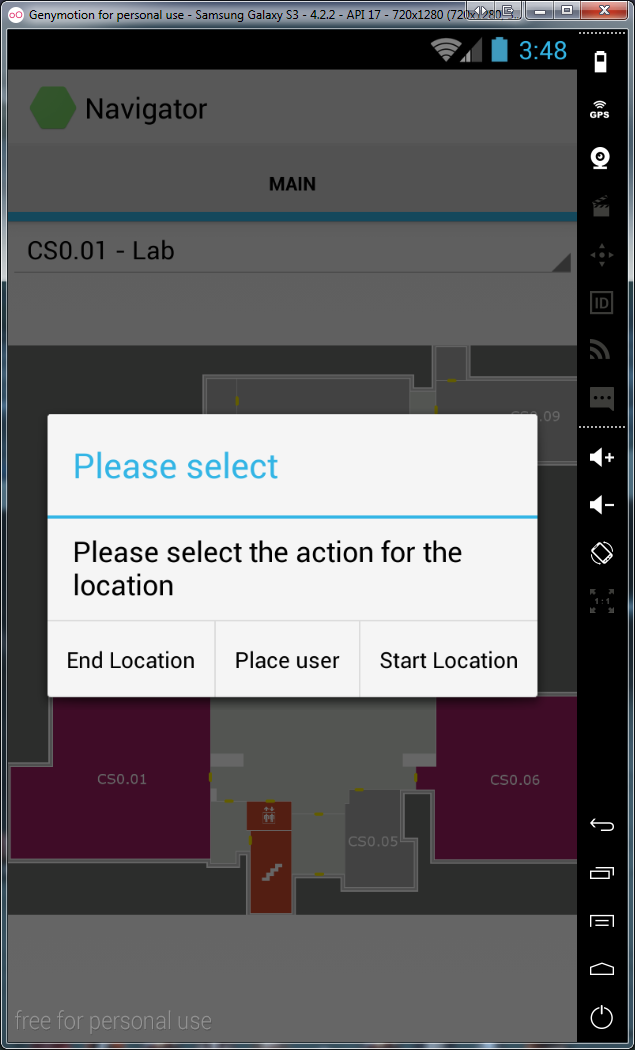
\includegraphics[scale=0.5]{images/location_action.png}
\captionof{figure}{Android start and end point selection menu.}
\label{fig:androidStartEndMenu}
\end{center}                    
                                    
                
        \subsection{Managing Points and Paths}
            Once the image was being displayed correctly and could be interacted with as required, the next step was to facilitate the drawing of start points, end points, the user location,
            and the path to follow on the screen. There were two approaches considered for this, the advantages and disadvantages of which are discussed below.
                \subsubsection{Overlay Based Approach}
                    This was the first of the approaches to be considered and involves the creation of a separate view to display the start/end points, user arrow, and path on top
                    of the floor plan image. Initially, this was an attractive solution as it allows the program to be constructed in a more modular way, keeping the management of the
                    floor plan apart from that of the drawing. However, it also introduces the additional task of managing the overlay itself. This becomes particularly challenging
                    when the user is scrolling around the floor plan or zooming in and out, due to the necessity of ensuring that the overlay view is also adjusted accordingly.
                    The other downside is that translating point coordinates from the overlay may also be tricky, perhaps requiring the use of another transformation matrix.
                    In the end, this method was deemed unsuitable for our purposes, so another solution was considered: directly editing the bitmap being displayed in the
                    \texttt{CustomImageView}.
                \subsubsection{Direct Bitmap Editing Approach}
                    This method involves editing the actual image being held in the image view. This approach addresses the primary issues found with the overlay based solution:
                    handling situations where the user wishes to either move or scale the floor plan by drawing the additional shapes into the bitmap image.
                     In this case, as the points and/or lines are part of the image itself, any translations
                    or scalings applied to the image as a whole will also, by extension, affect the points and lines. The downside to this approach is that it requires the image to be reset
                    to the default resource any time that a previously drawn point must be removed (such as moving a start point to a different location, or any movement of the
                    user arrow). It was thought initially that this may be a significant issue that could introduce a noticeable delay into interface updates, something that is clearly
                    unacceptable when a pleasant user experience is a key objective. Fortunately, some brief testing (on both emulators and physical Android devices)
                    revealed that this was not the case; there was no noticeable delay in interface updates. Following this discovery, it was decided to adopt this strategy instead of the
                    overlay system. The following section details how our custom helper class, \texttt{MapMaker}, handled the drawing of the required graphics.
                \subsubsection{MapMaker Helper Implementation}
                    \label{subsec:MapMaker}
                    The \texttt{MapMaker} class was created in order to keep the implementation of this part of the program separate from the rest of the application, in keeping
                    with the modular structure of most object-oriented programs. This meant that this module could be tested, maintained, and developed independently without 
                    adversely affecting the main activity -provided that changes to internal code did not alter the external behaviour of the class beyond what was intended.
                    
                    The first key component of this class was specifying the bitmap options that were applied to all of the decoded bitmaps (these being the plain floor plan,
                    the floor plan with the graph grid shown, and the user arrow).
                    The dither option is set to true in order to reduce noise in the image, in an attempt to prevent issues such as colour
                    banding. The bitmaps are also set to be purgeable i.e. the system can reclaim the memory used if absolutely necessary. In later versions of Android, this flag
                    is ignored, but enabling it allows a greater degree of backwards compatibility. Also note that enabling this did not prevent all memory issues, which will be discussed
                    later. The final key option was ensuring that the image is mutable. This is important as only mutable bitmaps can be used with Android
                    \texttt{Canvas} functionality, which enables the editing of the image i.e. only mutable images may be drawn into. In older versions, images could only be
                    made mutable by copying them, however this is inefficient in terms of both computation and memory, and is no longer the case for these very reasons.
                    
                    Upon initialising the instance of \texttt{MapMaker}, the class decodes and stores three android resources, all of which are bitmap images. These are the plain
                    floor plan, the floor plan with pathfinding grid, and the arrow used to display the current position of the user. The class provides functionality to clone
                    all of these bitmaps, which prevents the need to re-decode the images should a new blank copy of the image be required (such as when re-drawing the map
                    when erasing a point). This is beneficial performance-wise as decoding can be a slow process. As this redrawing has the potential to occur very frequently,
                    achieving good performance was of the utmost importance.
                    
                    Resetting the map was a simple process. When a call to \texttt{ResetMap} is made, a check is made to see if the grid is currently being drawn or not. Depending
                    on the result of this check, the correct bitmap can be cloned, edited, and then finally set as the current image being displayed by the view.
                    This function also makes sure to to call \texttt{Recycle} on the old bitmap image in order to ensure that the memory that it occupied is properly freed and
                    returned to the system at the next execution of garbage collection.
                    
                    Drawing into the bitmap was more complex, however. The bitmap is redrawn in the following situations:
                    \begin{itemize}
                        \item New start/end point selected.
                        \item User has taken a step, therefore the arrow must be moved.
                        \item The path must be (re-)drawn for some reason.
                    \end{itemize}
                    When a new start/end point is selected, the coordinates of this point are translated to coordinates in the bitmap via a transformation matrix
                    (discussed later in this section) and then stored within the \texttt{MapMaker}. Following this, a call is made to \texttt{DrawMap}, which first resets the
                    image (using \texttt{ResetMap}). Following this, the application forms a \texttt{Canvas} from the fresh image in order to facilitate the drawing of the
                    required shapes. Once this has been done, some simple checks are carried out in order to determine whether any start/end points are currently set.
                    If this is the case, the points are drawn at the previously stored coordinates using the \texttt{DrawCircle} function within \texttt{Canvas}. A similar check
                    is used to see whether the user arrow must also be drawn, if it must, the user arrow bitmap is also drawn into the \texttt{Canvas} by making use of
                    \texttt{DrawBitmap}. If both start and end points have been set, then the user path must also be drawn. Firstly, the correct nodes in the graph are obtained
                    by using the \texttt{FindClosestNode} function implemented within the \texttt{PathfindingGraph} object. These points are then passed to
                    \texttt{FindPath} in order to determine theh path to draw. Once the sequence of points has been calculated, the program iterates over this list, drawing lines
                    between adjacent points within the list using \texttt{DrawLine} until the end of the path is reached. Once all of the drawing has been completed, the
                    \texttt{Canvas} is disposed of in order to free memory. Finally, the image being displayed by the custom image view is updated to the newly edited
                    version.
                    
                    The final functionality that had to be added to this helper class was the ability to translate the coordinates of the location that a user has touched on the screen
                    into correct coordinates within the bitmap image. This was necessary due to the need to be able to place start and end points at a location specified by the user
                    performing a long press on the map via the device screen. The function takes either (\textit{x, y}) coordinates or a two-dimensional vector as input, and returns a
                    two-dimensional vector containing the newly translated coordinates. This is implemented by obtaining the image matrix from the custom image view and calculating
                    the inverse of this matrix. This new matrix can then be applied to the inputs in order to return the correctly translated coordinates. Figure  [~\ref{fig:androidPathDrawing}]  shows the android path drawing.

\begin{center}
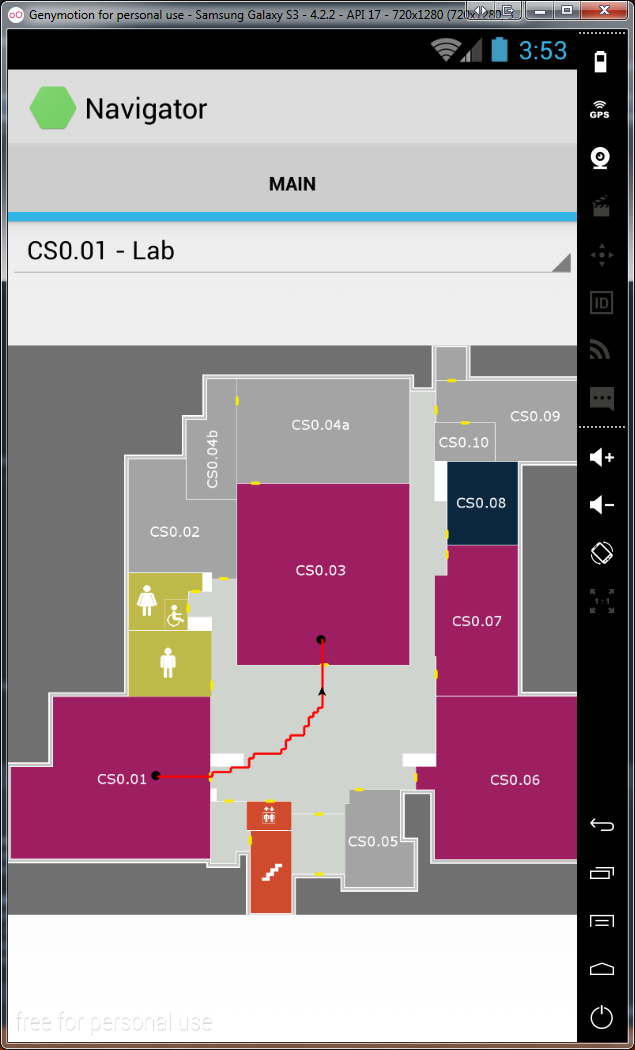
\includegraphics[scale=0.5]{images/pathfinding.png}
\captionof{figure}{Android path drawing.}
\label{fig:androidPathDrawing}
\end{center}
\end{document}
